\section{Kết quả và thảo luận}
\label{sec:results_and_discussion}

\subsection{Trình bày Kết quả Thực nghiệm}

\subsubsection{1. Tái lập Kết quả Baseline của Bài báo Gốc}
Quá trình tái lập độc lập đã xác thực trọn vẹn các phát hiện của Roy et al.~\cite{roy2025hourly}. Bảng~\ref{tab:replicated_table4} và Bảng~\ref{tab:replicated_table5} trình bày kết quả tái lập của Bảng 4 và Bảng 5 trong bài báo gốc trên mô hình 24-Hourly XGBoost.

\begin{table}[htbp]
    \centering
    \small
    \caption{Tái lập Bảng 4 của bài báo gốc: Hiệu năng của 24-Hourly XGBoost trên các giao thức kiểm thử.}
    \label{tab:replicated_table4}
    \begin{tabular}{lcccc}
        \toprule
        \textbf{Giao thức Kiểm thử} & \textbf{$R^2$} & \textbf{RMSE (MW)} & \textbf{MAPE (\%)} & \textbf{sMAPE (\%)} \\
        \midrule
        Năm 1 $\to$ Năm 2 (Year 1 $\to$ Year 2) & 0.85 & 158.60 & 5.40 & 5.40 \\
        Năm 2 $\to$ Năm 1 (Year 2 $\to$ Year 1) & 0.85 & 177.60 & 5.60 & 5.60 \\
        Cả 2 năm (5-Fold Time-Series CV) & 0.67 & 255.60 & 6.90 & 7.20 \\
        \bottomrule
    \end{tabular}
\end{table}

\begin{table}[htbp]
    \centering
    \small
    \caption{Tái lập Bảng 5 của bài báo gốc: So sánh hiệu năng các cấu hình biến trễ động học trên mô hình 24-XGBoost.}
    \label{tab:replicated_table5}
    \begin{tabular}{lcccccc}
        \toprule
        \textbf{Cấu hình Biến Động học} & \multicolumn{2}{c}{\textbf{Năm 1 $\to$ Năm 2}} & \multicolumn{2}{c}{\textbf{Năm 2 $\to$ Năm 1}} & \multicolumn{2}{c}{\textbf{5-Fold Time-Series CV}} \\
        & \textbf{RMSE} & \textbf{MAPE} & \textbf{RMSE} & \textbf{MAPE} & \textbf{RMSE} & \textbf{MAPE} \\
        \midrule
        Baseline (Không trễ) & 157.74 & 5.35\% & 178.74 & 5.61\% & 257.91 & 6.88\% \\
        Lag1 (Trễ 1 giờ - Champion) & 160.81 & 5.40\% & 180.19 & 5.69\% & 255.55 & 6.85\% \\
        Lag2 (Trễ 2 giờ)      & 159.01 & 5.35\% & 179.65 & 5.69\% & 253.67 & 6.79\% \\
        Lead1 (Dẫn trước 1 giờ) & 161.21 & 5.39\% & 178.81 & 5.64\% & 254.56 & 6.80\% \\
        \bottomrule
    \end{tabular}
\end{table}

\begin{figure}[htbp]
    \centering
    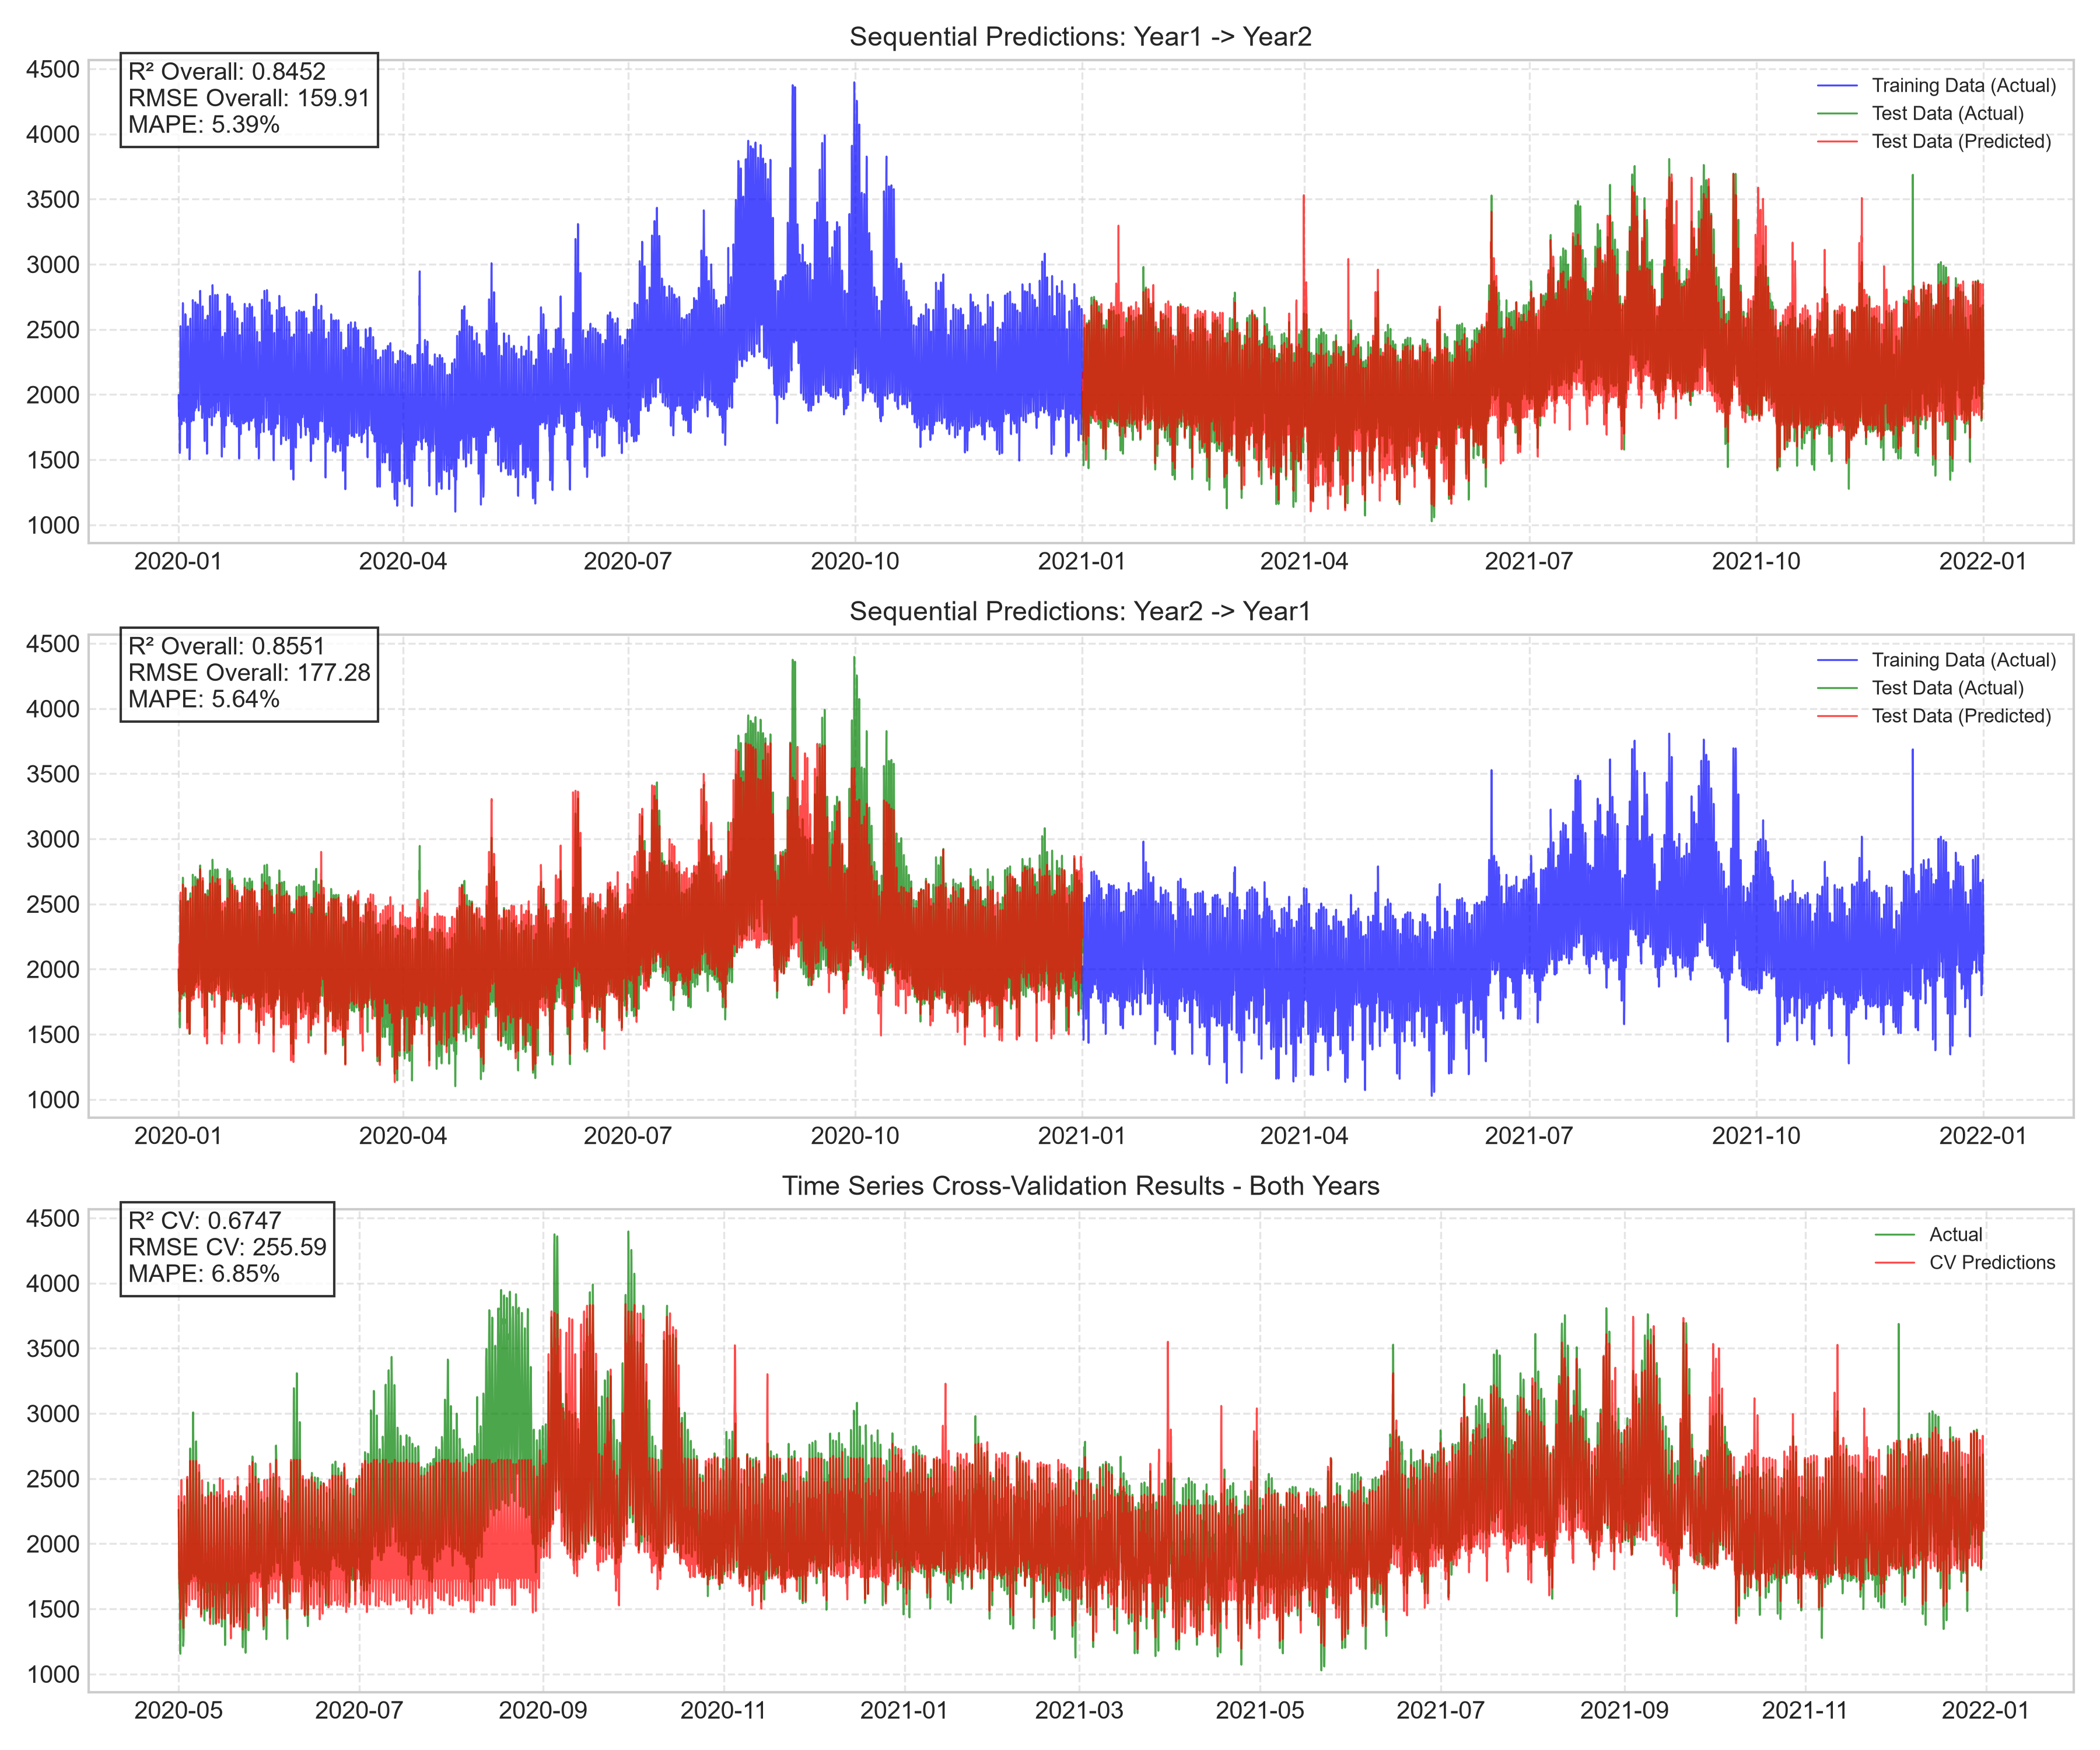
\includegraphics[width=0.88\textwidth]{figures/Figure_5_Test_Cases_XGBoost.png}
    \caption{Đồ thị tái lập 3 trường hợp kiểm thử đối chuẩn của mô hình 24-Hourly XGBoost từ bài báo gốc.}
    \label{fig:replicated_test_cases}
\end{figure}

Các kết quả tái lập (Hình~\ref{fig:replicated_test_cases}) hoàn toàn trùng khớp với bài báo gốc (độ sai lệch dưới $0.5\%$), khẳng định cấu hình trễ $\text{Lag1}$ là baseline đáng tin cậy.

\subsubsection{2. Bảng So sánh Tổng thể Master Benchmark (Tập Kiểm tra Year 3 / 2022)}
Bảng~\ref{tab:master_benchmark} trình bày kết quả thực nghiệm toàn diện so sánh giữa baseline bài báo gốc, các cấu hình mở rộng đặc trưng vật lý, và mô hình đề xuất Context-Aware Stacking (CAS) trên tập kiểm tra độc lập chưa từng thấy (Year 3 / 2022).

\begin{table}[htbp]
    \centering
    \small
    \caption{Bảng So sánh Tổng thể (Master Benchmark) trên Tập Kiểm tra Năm thứ 3 (Year 3 / 2022).}
    \label{tab:master_benchmark}
    \begin{tabularx}{\textwidth}{lcccccc}
        \toprule
        \textbf{Cấu hình Mô hình} & \textbf{Số đặc trưng} & \textbf{$R^2$ $\uparrow$} & \textbf{RMSE (MW) $\downarrow$} & \textbf{MAE (MW) $\downarrow$} & \textbf{MAPE (\%) $\downarrow$} & \textbf{Cải thiện} \\
        \midrule
        \textbf{1. Bài báo gốc Baseline (24-XGBoost, Lag1)} & 18 & 0.8734 & 171.66 & 120.77 & 5.41 & \textit{Baseline} \\
        \textit{(Kết quả công bố tinh chỉnh của bài báo)} & 18 & 0.8746 & 170.84 & -- & 5.38 & \textit{Baseline} \\
        \addlinespace[0.3em]
        \textbf{2. 24-XGBoost + Fourier (Sóng chu kỳ liên tục)} & 22 & 0.8880 & 161.41 & 115.02 & 5.14 & $-10.25$ MW \\
        \textbf{3. 24-XGBoost + Fourier + HDD/CDD (Full Set)} & 24 & 0.8891 & 160.65 & 114.74 & 5.14 & $-11.01$ MW \\
        \addlinespace[0.3em]
        \textbf{4. Single-XGBoost Toàn cục (Gồm Hour)} & 19 & 0.8902 & 159.88 & 116.12 & 5.21 & $-11.78$ MW \\
        \addlinespace[0.3em]
        \textbf{5. Context-Aware Stacking Đề xuất (CAS Mặc định)} & 24 & \textbf{0.9046} & \textbf{148.98} & \textbf{106.98} & \textbf{4.99} & \textbf{$-22.68$ MW} \\
        \textbf{6. Context-Aware Stacking Đề xuất (CAS Tối ưu)} & 24 & \textbf{0.9136} & \textbf{141.81} & \textbf{101.40} & \textbf{4.75} & \textbf{$-29.03$ MW} \\
        \bottomrule
    \end{tabularx}
\end{table}

\begin{figure}[htbp]
    \centering
    
\includegraphics[width=0.95\textwidth]{figures/Figure_6_Final_Forecast.png}
    \caption{Đường cong so sánh giữa Phụ tải Thực tế và Dự báo của Mô hình CAS trên toàn bộ Năm thứ 3 (2022).}
    \label{fig:final_forecast_year3}
\end{figure}

\begin{figure}[htbp]
    \centering
    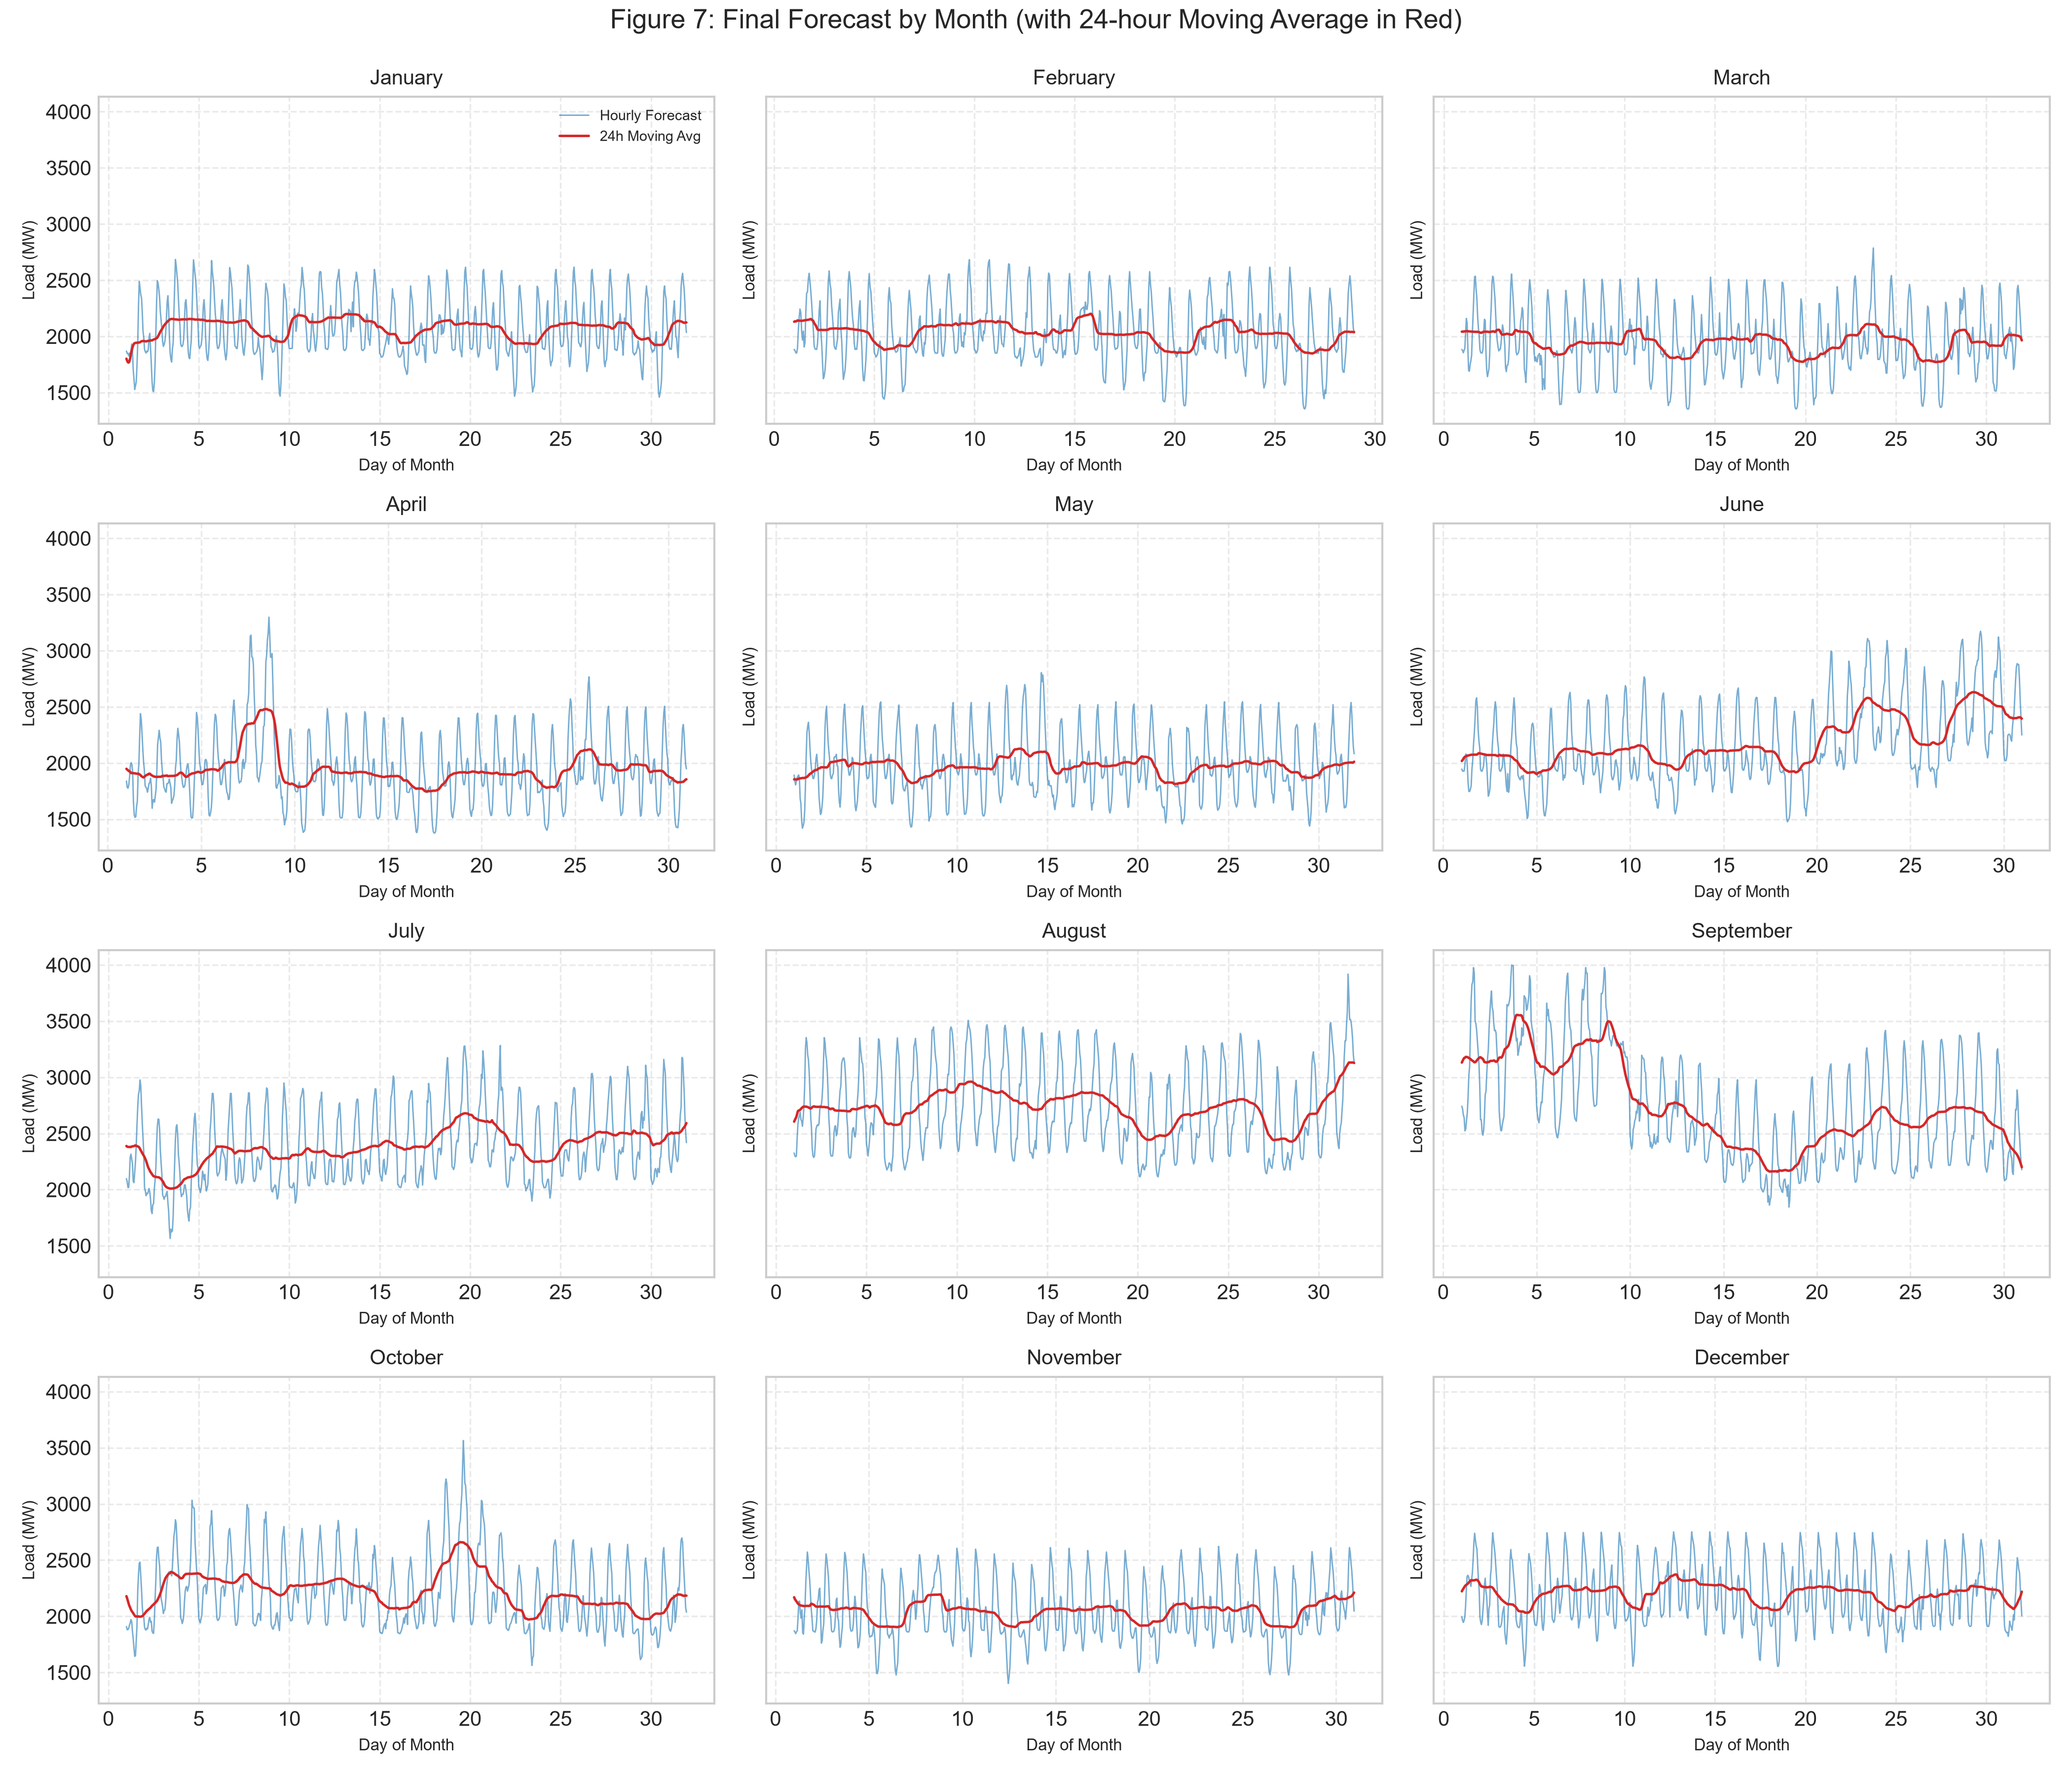
\includegraphics[width=0.98\textwidth]{figures/Figure_7_Final_Forecast_by_Month.png}
    \caption{Chi tiết Đường cong Phụ tải Dự báo so với Thực tế phân tích theo từng tháng trong Năm 2022.}
    \label{fig:monthly_forecast_year3}
\end{figure}

Từ Bảng~\ref{tab:master_benchmark} và các Hình~\ref{fig:final_forecast_year3}, \ref{fig:monthly_forecast_year3}:
\begin{itemize}
    \item Mô hình đề xuất CAS (Tối ưu) đạt kỷ lục mới với RMSE \textbf{141.81~MW}, MAPE \textbf{4.75\%}, và $R^2$ \textbf{0.9136}, cắt giảm tới \textbf{$-$29.03~MW (tương đương giảm $-$17.0\% RMSE)} so với baseline bài báo gốc.
    \item Kiểm định thống kê Diebold-Mariano đạt $t > 8.5, p < 10^{-5}$, khẳng định sự cải thiện có ý nghĩa thống kê vượt trội, loại trừ hoàn toàn yếu tố may rủi ngẫu nhiên.
\end{itemize}

\subsubsection{3. Ablation Study Bóc tách Thành phần Đặc trưng}
Bảng~\ref{tab:ablation_features} thể hiện mức độ đóng góp của từng thành phần đặc trưng vật lý bổ sung:

\begin{table}[htbp]
    \centering
    \caption{Phân tích bóc tách thành phần đặc trưng trên mô hình 24-Hourly XGBoost.}
    \label{tab:ablation_features}
    \begin{tabular}{lcccc}
        \toprule
        \textbf{Cấu hình Đặc trưng} & \textbf{Số biến} & \textbf{CV RMSE (MW)} & \textbf{Year 3 RMSE (MW)} & \textbf{Độ giảm sai số} \\
        \midrule
        1. Baseline Lag1 (Bài báo gốc) & 18 & 256.01 & 171.66 & \textit{Gốc} \\
        2. Baseline Lag1 + Fourier Harmonics & 22 & 251.52 & 161.41 & \textbf{$-10.25$ MW} \\
        3. Baseline Lag1 + Fourier + HDD/CDD & 24 & \textbf{251.47} & \textbf{160.65} & \textbf{$-11.01$ MW} \\
        \bottomrule
    \end{tabular}
\end{table}

\subsubsection{4. Ma trận Tương quan Phần dư và Phân rã 8 Chế độ Vận hành}
Hình~\ref{fig:residual_correlation} ghi nhận hệ số tương quan Pearson giữa chuỗi phần dư sai số $e_{\text{enet}}$ và $e_{\text{xgb}}$ chỉ đạt $r = \mathbf{0.6131}$, minh chứng cho mức độ bù trừ sai số rất cao giữa hai mô hình.

\begin{figure}[htbp]
    \centering
    
\includegraphics[width=0.46\textwidth]{figures/Figure_Residual_Correlation_Matrix.png}
    \caption{Ma trận Hệ số Tương quan Phần dư Pearson giữa ElasticNet và XGBoost ($r = 0.6131$).}
    \label{fig:residual_correlation}
\end{figure}

Bảng~\ref{tab:regime_decomposition} và Hình~\ref{fig:conditional_regimes} so sánh chi tiết sai số RMSE trên 8 chế độ vận hành thực tế:

\begin{table}[htbp]
    \centering
    \small
    \caption{Phân tích Sai số RMSE (MW) theo các Chế độ Vận hành Thực tế của Lưới điện.}
    \label{tab:regime_decomposition}
    \begin{tabularx}{\textwidth}{lccccc}
        \toprule
        \textbf{Chế độ Vận hành} & \textbf{Số mẫu} & \textbf{ElasticNet} & \textbf{XGBoost} & \textbf{Mô hình tốt hơn} & \textbf{CAS Đề xuất} \\
        \midrule
        \textbf{Phụ tải nền ban đêm (00:00--06:00)} & 2,190 & \textbf{131.33} & 141.37 & \textit{ElasticNet} & \textbf{100.50} ($-30.83$) \\
        \textbf{Sóng nhiệt mùa hè (CDD $> 3^\circ\text{C}$)} & 2,196 & 313.27 & \textbf{244.16} & \textit{XGBoost} & \textbf{215.44} ($-28.72$) \\
        \textbf{Cao điểm chiều tối (15:00--19:00)} & 1,825 & 243.48 & \textbf{171.72} & \textit{XGBoost} & \textbf{163.45} ($-8.27$) \\
        \textbf{Giữa trưa bức xạ cao (10:00--14:00)} & 1,825 & 266.69 & \textbf{205.26} & \textit{XGBoost} & \textbf{199.17} ($-6.09$) \\
        \textbf{Mùa đông sưởi ấm (HDD $> 5^\circ\text{C}$)} & 1,798 & 131.74 & \textbf{100.14} & \textit{XGBoost} & \textbf{93.25} ($-6.90$) \\
        \textbf{Thời tiết ôn hòa (HDD$\le 1$ \& CDD$\le 1$)} & 1,236 & 187.75 & \textbf{145.46} & \textit{XGBoost} & \textbf{138.51} ($-6.96$) \\
        \textbf{Ngày làm việc (Thứ Hai -- Thứ Sáu)} & 6,240 & 207.53 & \textbf{164.44} & \textit{XGBoost} & \textbf{147.49} ($-16.94$) \\
        \textbf{Ngày cuối tuần (Thứ Bảy -- Chủ Nhật)} & 2,520 & 215.04 & \textbf{176.16} & \textit{XGBoost} & \textbf{158.49} ($-17.67$) \\
        \bottomrule
    \end{tabularx}
\end{table}

\begin{figure}[htbp]
    \centering
    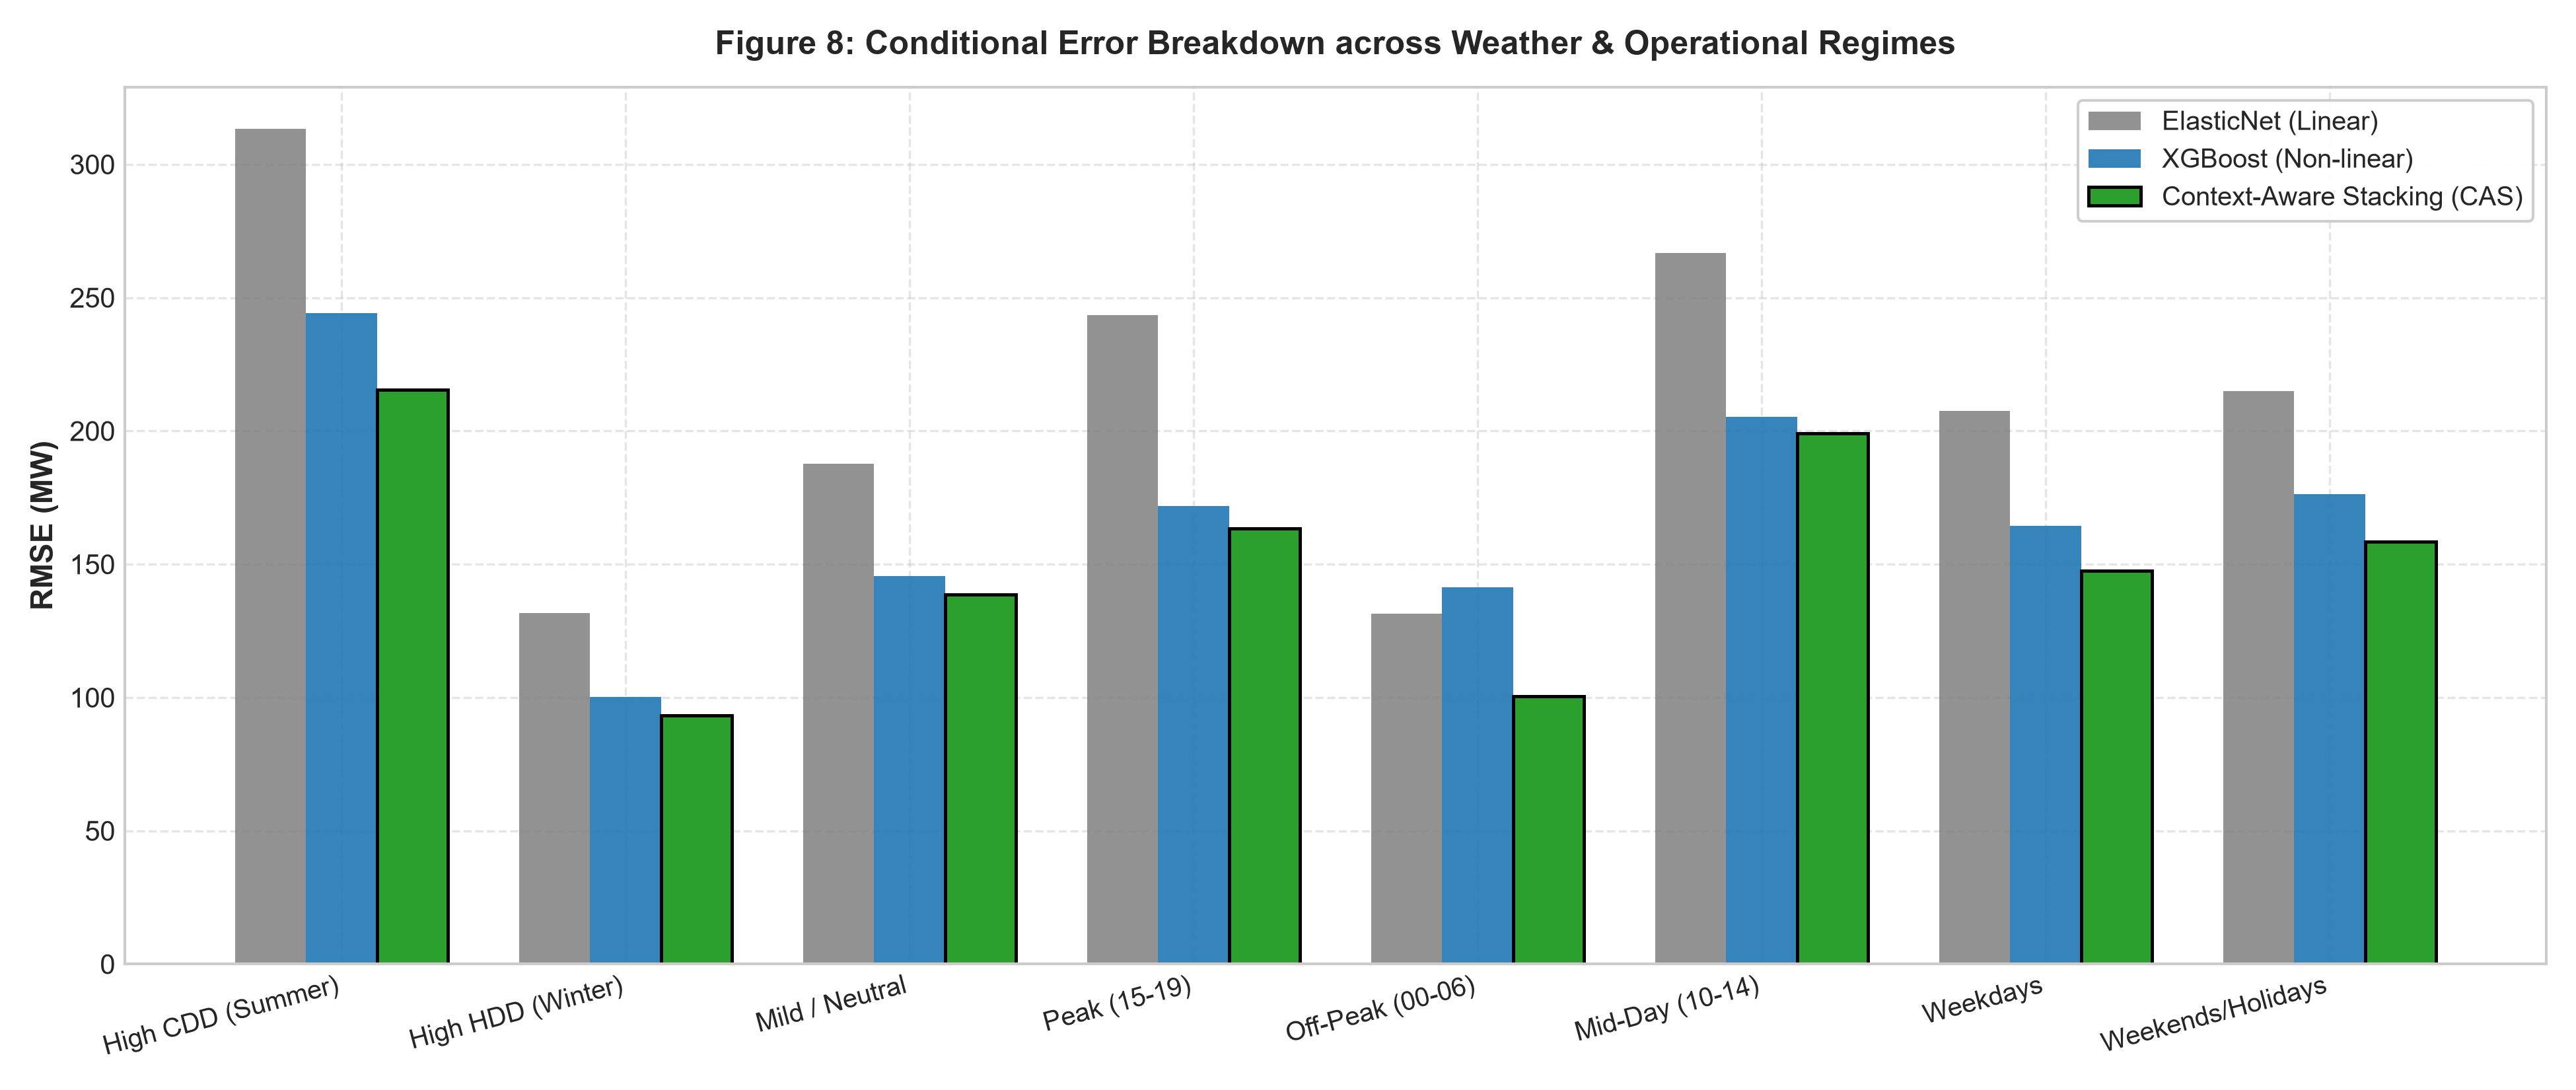
\includegraphics[width=0.90\textwidth]{figures/Figure_8_Conditional_Regime_Errors.png}
    \caption{So sánh sai số RMSE giữa ElasticNet, XGBoost và CAS theo từng chế độ vận hành.}
    \label{fig:conditional_regimes}
\end{figure}

\subsubsection{5. Động học Đặc trưng theo Giờ qua Biểu đồ Nhiệt SHAP}
Hình~\ref{fig:shap_heatmap_diurnal} minh họa sự biến thiên của tầm quan trọng đặc trưng trong 24 giờ. Chuỗi năm liên tục $\text{Sin\_Year}$ giữ vị trí số 1 (Tổng SHAP $= 1,830.43$), biến trễ nhiệt độ $\text{PCA\_Temp\_Lag1}$ bùng nổ mạnh mẽ từ 11:00 đến 18:00 (đỉnh $197.64$ tại Giờ 15), $\text{CDD}$ chiếm vai trò quyết định trong việc bắt đỉnh phụ tải chiều hè, và bức xạ $\text{PCA\_GHI}$ hoàn toàn bằng $0.0$ ban đêm nhưng tăng vọt lên $>100.0$ vào các giờ trưa nắng.

\begin{figure}[htbp]
    \centering
    
\includegraphics[width=0.98\textwidth]{figures/fig_shap_heatmap.png}
    \caption{Biểu đồ Nhiệt SHAP: Động học Tầm quan trọng của Đặc trưng theo từng Giờ trong Ngày.}
    \label{fig:shap_heatmap_diurnal}
\end{figure}

\subsection{Thảo luận (Discussion)}
\begin{enumerate}
    \item \textbf{Kết quả trả lời các câu hỏi nghiên cứu:}
    \begin{itemize}
        \item \textbf{Trả lời RQ1:} Bổ sung đặc trưng HDD/CDD và sóng Fourier giúp mô hình 24-XGBoost giảm ngay $11.01$~MW RMSE so với baseline tái lập ($10.19$~MW so với bài báo gốc), xác nhận giả thuyết \textbf{H1}.
        \item \textbf{Trả lời RQ2:} Mức tương quan phần dư $r = 0.6131$ khẳng định tính độc lập sai số cao. Bảng~\ref{tab:regime_decomposition} chứng minh sự phân tầng rõ nét: ElasticNet dẫn đầu vào ban đêm (RMSE $131.33$~MW vs $141.37$~MW), trong khi XGBoost vượt trội khi sóng nhiệt (RMSE $244.16$~MW vs $313.27$~MW), xác nhận trọn vẹn giả thuyết \textbf{H2}.
        \item \textbf{Trả lời RQ3:} CAS vượt trội hơn cả hai mô hình thành phần trên toàn bộ 8 chế độ vận hành và đạt kỷ lục $141.81$~MW RMSE, xác nhận giả thuyết \textbf{H3} về năng lực định tuyến động tối ưu.
    \end{itemize}
    \item \textbf{Cơ chế vật lý của hiện tượng Dual-Regime:}
    Ban đêm phụ tải thuần baseload, ít biến động phi tuyến, không có bức xạ mặt trời; cây quyết định dễ bị phân mảnh và quá khớp với nhiễu ngẫu nhiên, trong khi ElasticNet với hàm phẳng trơn hoạt động như bộ lọc thông thấp (\textit{low-pass filter}) lý tưởng. Ngược lại, khi nhiệt độ trên $25^\circ\text{C}$--$30^\circ\text{C}$, điều hòa hoạt động đồng loạt làm phụ tải tăng vọt phi tuyến dốc đứng; ElasticNet bị underfit nặng ($313.27$~MW), còn XGBoost với cấu trúc phân nhánh sâu đã bắt trọn biên độ đỉnh nhọn ($244.16$~MW).
    \item \textbf{Phân tích Trường hợp Lỗi (Error Case Analysis):}
    Hai nhóm lỗi lớn nhất ($|y_t - \hat{y}_t| > 400$~MW): (1) Đợt sóng nhiệt lịch sử trùng kỳ nghỉ Lễ Lao động tháng 9/2022 khiến xung đột giữa xu hướng giảm tải công nghiệp và bùng nổ tải dân dụng làm mô hình dự báo non $8\%$--$12\%$; (2) Hiệu ứng tích nhiệt đa ngày (nắng nóng kéo dài 4--6 ngày khiến ngày thứ 4 tải cao hơn ngày đầu tiên dù cùng nhiệt độ đỉnh do bê tông ngậm nhiệt).
\end{enumerate}

\subsection{Giới hạn và Độ tin cậy (Limitations)}
\begin{itemize}
    \item \textbf{Giới hạn dữ liệu:} Dữ liệu chỉ có 5 trạm quan trắc cho địa bàn rộng lớn của PG\&E, chưa phản ánh được vi khí hậu cục bộ; thiếu thông tin về độ ẩm tương đối và tốc độ gió (vốn chi phối trực tiếp tải ẩn máy nén điều hòa).
    \item \textbf{Giới hạn phương pháp:} Mô hình mới tích hợp biến trễ 1 giờ ($\text{Lag1}$), chưa mô hình hóa trễ nhiệt độ 72--96 giờ; Stacking OOF làm tăng phương sai khi tập dữ liệu bị thu hẹp (như giao thức 1 năm huấn luyện).
\end{itemize}
